% Preamble starts
% ---------------
\documentclass{article}
\usepackage{geometry}
\geometry{
 a4paper,
 left=30mm,
 right=30mm,
 top=30mm,
 bottom=30mm,
 }
\newcommand{\HorRule}{\color{Black}\rule{14cm}{1pt}} % Defines the gold horizontal rule around the title
\usepackage[utf8]{inputenc}
\usepackage[dvipsnames]{xcolor}
\pagenumbering{arabic}
\usepackage{amsmath}
\usepackage{amsthm}
\usepackage{amssymb}
\usepackage{graphicx}
\usepackage{url}
\usepackage[titletoc,title]{appendix}
\linespread{1.3}
\newtheorem{definition}{Definition}[section]
\newtheorem{result}[definition]{Result}
\newtheorem{theorem}{Theorem}[section]
\newtheorem{corollary}{Corollary}[theorem]
\newtheorem{lemma}[theorem]{Lemma}
% ---------------

% Document Starts
% ---------------
\begin{document}

% Title page
\begin{titlepage}
   \begin{center}
        \vspace*{2cm}
        \LARGE
        \textbf{COMP0120 Numerical Optimisation}

        \Large
        \vspace{1cm}
        Assignment 2
        \vspace{0.5cm}
        \HorRule
        
        \vspace{4cm}
        \textbf{Lagrangian Support Vector Machines}

        \large
        \vspace{4cm}
        \HorRule
        \vspace{1cm}
        \textit{Date:\\} \textbf{April 2022} \\
        \vspace{0.5cm}
        \textit{Word Count:\\} \textbf{2946} \\ \text{(\LaTeX)}
            
   \end{center}
\end{titlepage}

% Question 1
\section{Question 1}
%\setlength{\parindent}{2em}
%\setlength{\parskip}{1em}

% ----------
% Part (a)
% ----------
\subsection*{\textbf{Q1 – Part (a)}}
\normalsize

For this project we have chosen to use a subset of the Dry Bean dataset provided by the UCI Machine Learning Repository \cite{misc_dry_bean_dataset_602}. This subset comprises of all 16 features of the data, but only two of the registered dry bean categories: SIRA \{+1\} and DERMASON \{–1\}, to restrict our classification problem to the binary case. This left us with approximately 7,000 datapoints. \par

We have sought to find an optimal hyperplane that separates the two dry bean categories using a Support Vector Machine (SVM) Algorithm. We have split the data 80/20 into a training and testing set. The training set will be used in the optimisation problem, the testing set will be reserved for performance analysis against the classifications predicted by our SVM.

% ----------
% Part (b)
% ----------
\subsection*{\textbf{Q1 – Part (b)}}
The most appropriate formulation for our SVM classification task is the dual with a non-linear kernel and slightly modified non-standard loss function. \par

We have chosen to optimise the dual function as it reduces to a far simpler problem than the initial primal, with fewer constraints. Since the data is non-separable, we can use the so called `kernel trick' \cite{scholkopf1997kernel, scholkopf1998nonlinear} to transform our dataset into a higher dimensional feature space, seek a separating hyperplane there, and then transform back to our original space to improve the classification. \par 

For our problem, we used a homogeneous quadratic polynomial kernel.
\begin{definition} \textbf{Homogeneous Quadratic Polynomial Kernel} \cite{shashua2009introduction} \\
Let $x_{i}, x_{j} \in \mathbb{R}^{m}$ be arbitrary vectors from the input space. Then the homogeneous quadratic polynomial kernel is defined as,
\begin{equation}
    K(x_{i},x_{j}) = (x_{i}^{T}x_{j})^2.
\end{equation} 
\end{definition} \par

Similarly, we will use the following modified standard loss function.
\begin{definition} \textbf{Squared Standard Loss Function} \cite{scholkopf2002learning:ch3} \\
Let $x$ be an input in the feature space, $y$ the true classification output, and $f(x)$ a classification prediction based on input $x$. Then the squared standard loss function is defined as,
\begin{equation}
    c(x, y, f(x)) = max(0, 1-yf(x))^2.
\end{equation}
\end{definition} \par

To understand why we have used this, let us first consider the traditional soft margin SVM optimisation with the standard loss function. 

\begin{definition} \textbf{Soft Margin Optimal Hyperplane (Primal Function)} \cite{vapnik1999nature:ch5}\\
Define $\mathcal{H} \subset \mathbb{R}^m$ to be a dot product space. Let $\textbf{w} \in \mathcal{H}, b \in \mathbb{R}$, and $C$ $\geq$ 0. Then we can introduce non-negative slack variables $\xi_{i} \geq$ 0 for $i = 1, \ldots, m$ such that our soft margin classifier can be found by minimising the objective function,
\begin{equation}
    \min_{\textbf{w} \in \mathcal{H}, \xi \in \mathbb{R}^m} {\tau(\textbf{w}, \xi) = \frac{1}{2} \|\textbf{w}\|^2 + C \sum_{i=1}^{m} \xi_{i}}.
\end{equation}
Subject to the constraints,
\begin{equation}
    y_i (\textbf{w} \cdot \mathbf{x_{i}} + b) \geq 1  -\xi_{i} , i=1, \dots, m
\end{equation}
\begin{equation}
    \xi_{i} \geq 0.
\end{equation}
\end{definition}

Which, in turn, leads to the following definition of the associated dual. 
\begin{definition} \textbf{Dual Function} \cite{vapnik1999nature:ch5}\\
Let $\lambda_i$ be Lagrange multipliers and $K$ represent our kernel function. Then the corresponding dual function is,
\begin{equation}
    \min_{\lambda \in \mathbb{R}^m} {\frac{1}{2}} \sum_{i=1}^{m} \sum_{j=1}^{m} \lambda_{i} \lambda_{j} y_{i} y_{j} K(x_{i}, x_{j}) - \sum_{i=1}^{m} \lambda_{i}
\end{equation}
Subject to the constraints,
\begin{equation}
   0 \leq \lambda_{i} \leq \frac{C}{m} \text{ for all } i=1, \ldots, m 
\end{equation}
\begin{equation}
    \sum_{i=1}^{m}{\lambda_{i} y_{i} = 0}.
\end{equation}

\end{definition}

This is a rather complicated form, containing both bounded constraints (7) and equality constraints (8). In addition, it can be shown (by writing the dual function (6) in equivalent matrix form) that, in general, this formulation is not positive definite \cite{mangasarian1999successive} since $m >> n$, as is the case for our classification problem. \par

Techniques exist that can solve optimisation problems of this kind, such as Sequential Minimal Optimisation (SMO) \cite{platt1998sequential} or SVM-\textit{light} \cite{joachims1999svmlight}, however, if we alter the initial formulation of the Primal function (3) by including the proposed non-standard loss (2) and including an additional term in the objective function, we can simplify the problem even further. This allows us to use an alternative, iterative method: the Lagrangian Support Vector Machine (LSVM) Algorithm \cite{mangasarian2001lagrangian}. 


% ----------
% Part (c)
% ----------
\subsection*{\textbf{Q1 – Part (c)}}    
We shall now introduce the new formulation. Overall, there are two changes proposed:
	\begin{enumerate} 
	    \item[(i)]
	    The squared loss function leads us take the square of the slack variables $\xi_{i}$. This means we no longer need to consider the non-negativity constraint (5).
	    \item[(ii)]
	    We introduce the term $b^2$ into our primal objective function. This means we are now seeking to optimise with respect to both the orientation ($\textbf{\textit{w}}$) and location ($b$) of the hyperplane \cite{mangasarian1999successive}.
	\end{enumerate}

These conditions introduce a new primal and associated dual.

\begin{definition} \textbf{Modified Primal Function} \cite{scholkopf2002learning:ch10}\\
Let $\textbf{w} \in \mathcal{H}$, $b \in \mathbb{R}$, $\xi \in \mathbb{R}^m$, and $\nu > 0$. Define $\phi (x)$ as the transformation associated with the kernel $K$. Then the modified primal function is defined as,
\begin{equation}
    \min_{w, b, \xi} = \frac{\nu}{2} \sum_{i=1}^{m} \xi_i + \frac{1}{2} ( \| \textbf{w} \|^2 + b^2).
\end{equation}
Subject to the constraint,
\begin{equation}
    y_i ( \textbf{w} \cdot \phi(\mathbf{x_{i}}) + b) \geq 1  -\xi_{i} \text{ for all } i=1, \dots, m.
\end{equation}
\end{definition}

And once more, the associated modified dual. 
\begin{definition} \textbf{Modified Dual Function} \cite{scholkopf2002learning:ch10} \\
Let $\delta_{ij}$ represent the Kronecker delta, and $K_{ij}$ the $ij^{th}$ component of the kernel (or Gram) matrix. Then the modified dual function is,
\begin{equation}
    \min_{\lambda \in \mathbb{R}^m} {\frac{1}{2}} \sum_{i=1}^{m} \sum_{j=1}^{m} \lambda_{i} \lambda_{j} y_{i} y_{j} (K_{ij} + 1 + \frac{1}{\nu} \delta_{ij}) - \sum_{i=1}^{m} \lambda_{i}
\end{equation}
Subject to the constraint,
\begin{equation}
    \lambda_{i} \geq 0.
\end{equation}
\end{definition}

Whilst the objective function appears more complicated in our modified dual (11) than in our original (6), the constraints have been dramatically simplified. Furthermore, we have a simple relation between the dual parameters and the primal variables.
\begin{align}
    \textbf{\textit{w}} &= \sum_{i=1}^{m} y_{i} \lambda_{i} \phi(x_{i}), \\
    b &= \sum_{i=1}^{m} \lambda_{i}, \\
    \xi_{i} &= \frac{\lambda_{i}}{\nu}.
\end{align}


This is the formulation considered throughout this project.

% ----------
% Part (d)
% ----------
\subsection*{Q1 – Part (d)}
Both our modified primal and dual functions are convex. This can be seen from the following definitions and results. \par

\begin{definition} \textbf{Dot Product Space} \cite{scholkopf2002learning:appendix} \\
The dot product space $\mathcal{H}$ is a symmetric bilinear form that is strictly positive definite. That is, for all $\textbf{x} \in \mathcal{H}$, we have that $(\textbf{x} \cdot \textbf{x}) \geq 0$. 
\end{definition}

\begin{definition} \textbf{Convex Combinations} \cite{scholkopf2002learning:appendix} \\
Given a real vector space, $\mathcal{H} \subset \mathbb{R}^{m}$, we can construct convex combinations for any $\textbf{x} \in \mathcal{H}$,
\begin{equation}
    \sum_{i=1}^{m} \lambda_{i} \textbf{x}_{i}.
\end{equation}
Where, 
\begin{align}
    \lambda_{i} \geq 0, \text{ and, }
    \sum_{i=1}^{m} \lambda_{i} = 1.
\end{align}
\end{definition}

\begin{result}
        Every norm is a convex function.
\end{result} 
\begin{proof}
    See \cite{web:maths:UCL}
\end{proof}

As we have seen, our vector $\textbf{\textit{w}}$ is defined on the dot product space $\mathcal{H}$ for both our primal (9) and dual (11) functions. In addition the primal includes the norm in the objective function. Finally, our dual is clearly a convex combination of the Lagrange multipliers $\lambda_{i}$ and classifications $y_{i}$. \par

The fact that our objective function is convex leads to some nice properties. The most important of which is that \textit{any local minimum is also a global minimum} \cite{web:maths:princeton}. This property will be used when we discuss convergence in Q2.\par

Unfortunately, there are still some challenges with our reformulation. As we will see shortly, the iterative nature of the method requires the inversion of a large matrix (albeit only once). In addition, by introducing the $b^2$ term into the objective function, we are essentially applying regularisation and as a result lose translation invariance in the feature space \cite{scholkopf2002learning:ch10}.

\newpage
\section{Question 2}

% ----------
% Part (a)
% ----------
\subsection*{\textbf{Q2 – Part (a)}}
As has already been alluded to, we propose the Lagrangian Support Vector Machine Algorithm \cite{mangasarian2001lagrangian} to solve our classification problem. This method is applicable for several reasons. Firstly, our modifications leading to the dual function (11) allow us to use an iterative approach to identifying the optimal Lagrange multipliers and the direct relation between the dual parameters and the optimal hyperplane mean we can easily recover our solution. Furthermore, we can see from (11) that the dual formulation includes an arbitrary non-linear kernel $K_{ij}$, hence, we need only change the Kernel matrix in our algorithm to account for non-linearity. \par

The reformulation has the additional benefit of being globally convergent, which removes issues faced by Newton methods, in which not every initial point is feasible \cite{boyd2004convex}.
As this is a small to intermediate classification problem (the number of datapoints is in the region $10^{3} - 10^{4}$) we also seek an appropriate rate of convergence – at least linear – which, as we shall see in part (d), the algorithm satisfies. \par

Finally, the iterative solution of the dual only requires the inversion of a matrix once, during the initial setup. This is particularly useful as it means the CPU time is minimal and the memory usage is reduced – especially if we can find a low rank approximation of the kernel matrix, and approximate the inverse, thus further reducing the computational effort required. 

% ----------
% Part (b)
% ----------
\subsection*{\textbf{Q2 – Part (b)}}
To simplify our notation, increase readability, and rely on matrix multiplication during the implementation of our code, we rewrite the dual function (11) once more. \par

Firstly, let $A$ refer to the input matrix, that is the matrix consisting of $m$ rows (\textit{number of points in the dataset}) and $n$ columns (\textit{the features of the dataset}).
We can then define a new matrix,
\begin{equation}
    H := [A, -\Vec{1}].
\end{equation}
Where we have appended a vector $-\Vec{1}$ onto $A$. This takes care of the $K_{ij} + 1$ term in (11). The difference in sign is due to the fact that in (11) we are computing the kernel matrix from the input $A$ and then adding one, whereas in (18) we are forming a new input matrix $H$, then applying the kernel transformation to form the kernel matrix. By doing so we can reorder the terms of our expression whilst maintaining appropriate matrix multiplication. \par
Let $K$ be a map taking two matrices and applying the kernel transformation, such that for our homogeneous quadratic polynomial kernel we have, 
\begin{equation}
    K(H,H^{T}) = (H H^{T})^2.
\end{equation} 
Where the square refers to the element-wise square, with a slight abuse of notation. Finally, we shall define $D := \text{diag}(y)$.

These changes simply allow us to write the dual in an equivalent matrix form rather than index form. We now have,
\begin{equation}
    \min_{\lambda \in \mathbb{R}^{m}} {\frac{1}{2} \lambda^{T} (\frac{I}{\nu} + DK(H, H^{T})D) \lambda - \Vec{1}^{T} \lambda }.
\end{equation}
Subject to the same constraint as (12),
\begin{equation*}
    \lambda_{i} \geq 0.
\end{equation*}

For what follows we will further define,
\begin{equation}
    M := (\frac{I}{\nu} + DK(H, H^{T})D).
\end{equation}

So far, we have only been manipulating the objective function. To solve the problem, we must now consider the KKT optimality conditions for (20). We have seen from the lectures that our Lagrange multipliers, $\lambda$, are only non-zero if the constraints described in (10) are active. 

Using the definition of $M$ (21), Mangasarian \cite{mangasarian1994nonlinear} showed the KKT necessary and sufficient optimaility condition for our dual equation (20) is simply,
\begin{equation}
    \lambda^{T} (M \lambda - \Vec{1}) = 0.
\end{equation}
Which allows us to introduce the following Lemma.

\begin{lemma} \textbf{Orthogonality \& Clipping} \\
Let us define two arbitrary vectors $a, b \in \mathbb{R}^m$. Then we have the two following equivalent conditions.
\begin{equation}
    \{a, b \geq 0 \text{ and } a^{T}b = 0\} \Longleftrightarrow \{a = (a-\tau b)_{+} \text{ for all } \tau > 0\}
\end{equation}
\end{lemma}
\begin{proof}
See \cite{scholkopf2002learning:ch10}.
\end{proof}

The direct consequence of Lemma 2.1. is that the KKT conditions (22) can be equivalently written as,
\begin{equation}
    (M \lambda - \Vec{1}) \Longleftrightarrow ((M \lambda - \Vec{1}) - \tau \lambda)_{+} \text{ for all } \tau > 0.
\end{equation}

This follows as we have simply substituted $a = (M \lambda - \Vec{1})$ and $b = \lambda$ into Lemma 2.1, and used the fact that $a^{T}b = b^{T}a$. \par

As a result, this provides the iterative step for our LSVM Algorithm,
\begin{equation}
    \lambda_{i+1} = M^{-1}(((M \lambda_{i} -\Vec{1}) -\tau \lambda_{i})_{+}) + \Vec{1}).
\end{equation} \par

From (25), it is clear we require the inverse of the matrix $M$. Let us now turn our attention to methods of forming $M^{-1}$ in a computationally efficient way. We are faced with two scenarios. \par

\textbf{Scenario 1: Best Case} \\
If the circumstances permit, we can use a special case of the  Sherman-Woodbury-Morrison formula devised by Golub and Van Loan \cite{golub2013matrix}, which reduces the complexity of the inversion required from an $m \times m$ matrix, to a $k \times k$ matrix, with $k << m$. 
We repeat the formula here. \par

Let $\Lambda \in \mathbb{R}^{m \times k}$ be an arbitrary matrix, then
\begin{equation}
    (\frac{I}{\nu} + \Lambda \Lambda^{T})^{-1} = \nu(I - \Lambda(\frac{I}{\nu} + \Lambda^{T} \Lambda)^{-1} \Lambda^{T}).
\end{equation} \par

It is clear that (26) is simply a generalised case of what we have defined as $M$ in (21). \par 

Alternatively, we can preempt our use of the kernel $K$ by applying a low-rank approximation of the kernel transformation applied to our input matrix $A$ \cite{scholkopf2002learning:ch10}.
\begin{equation}
    A \rightarrow K^{m \times n}(K^{n \times n})^{-\frac{1}{2}}.
\end{equation}
Where the indices of $K$ represent the matrix dimensions. \par

Unfortunately, however, these tricks require us to: (a) know the inner product terms of the kernel (which in general are not known); and (b) find a low-rank approximation of the kernel transformation (which in general is difficult). \par

\textbf{Scenario 2: Traditional Case} \\
Sadly, the two drawbacks mentioned previously are present in our classification problem, meaning we cannot use such tricks. This further reinforces the fact that the LSVM Algorithm is only applicable up to and including intermediate sized problems. To invert our matrix then, we must resort to traditional LU decomposition (present in the MATLAB \textit{inv($\cdot$)} function) \cite{web:maths:MATLAB} in a similar manner to interior-point algorithms.


% ----------
% Part (c)
% ----------
\subsection*{Q2 – Part (c)}
To discuss the convergence type and rate, we will use Lemma 2.1. Formally, both the \textit{type} and \textit{rate} are combined into a single theorem, we shall separate the two and discuss each element individually.

\begin{theorem} \textbf{Convergence \textit{type} of the LSVM Algorithm} \cite{mangasarian2001lagrangian} \\
Under the assumption that $K$ and $M$ are positive symmetric matrices, and the following condition on tau holds,
\begin{equation}
    0 \leq \tau \leq \frac{2}{\nu}.
\end{equation}
Then given an arbitrary starting point $\lambda_{0}$ our iterative scheme will converge to the solution $\lambda^{*}$.
\end{theorem}
\begin{proof}
The proof by Mangasarian and Musicant uses the Projection Theorem \cite{bertsekas1997nonlinear} and  bounds the alternative definition of the optimality conditions (24) using the Cauchy-Schwarz inequality.
\end{proof}

Aside from the rather trivial fact that the proof for both the rate and type of convergence was developed simultaneously alongside the algorithm itself, we can confirm that the result does indeed apply to our problem. \par

We first require that $K$ and $M$ are positive symmetric matrices. As it so happens, this occurs by construction. Throughout the modifications leading to the dual (11), we have assumed an arbitrary input matrix $A$, which is substituted into $H$ (18) and transformed using the map $K$ (19). It was shown by Mangasarian \cite{mangasarian1994nonlinear} that our definition of $M$ (21) was thus symmetric positive definite, and likewise for $K$ (since it is a component of $M$). Naturally, by extension, these assumptions hold for our problem since they hold for an arbitrary input matrix $A$ and kernel map $K$. \par

Turning our attention to (28), at first glance it may appear a rather unusual assumption. However, once again by construction, $\nu > 0$ and therefore $\frac{1}{\nu}$ specifies the smallest eigenvalue of our matrix $M$. This means that our parameter $\tau$ which feeds into the KKT optimality condition (24), and thus the iterative step (25), cannot be an eigenvalue of $M$ and hence prevents the algorithm from breaking down. In the context of our problem, $\nu$ is a parameter that is parsed by the user, so this assumption also holds. \par

Furthermore, as we noted in Q1 – Part (d), our dual function (11) is convex, thus any local minimum is also a global minimum. Since all the assumptions of Theorem 2.2 are satisfied and applicable to our problem, these two results combine to dictate the type of convergence we can expect. Our arbitrarily chosen starting value for the iterative scheme of Lagrange multipliers $\lambda_{0}$ will converge. Hence, the LSVM Algorithm is globally convergent.

% ----------
% Part (d)
% ----------
\subsection*{Q2 – Part (d)}
As mentioned, the rate of convergence is also captured in the same formal Theorem. We now present the second part.
\begin{theorem} \textbf{Convergence \textit{rate} of the LSVM Algorithm} \cite{mangasarian2001lagrangian} \\
Under the assumption that $K$ and $M$ are positive symmetric matrices, and the following condition on tau holds,
\begin{equation}
    0 \leq \tau \leq \frac{2}{\nu}.
\end{equation}
Then given an arbitrary starting point $\lambda_{0}$ our iterative scheme will converge to the solution $\lambda^{*}$ at a linear rate, and consequently,
\begin{equation}
    \frac{\|M \lambda_{i+1} - M \lambda^{*} \|}{\|M \lambda_{i} - M \lambda^{*} \|} \leq \| I - \tau M^{-1} \|.
\end{equation}
\begin{proof}
The result (30) is a direct consequence of Mangasarian and Musicant's proof of Theorem 2.2, where we have used the alternative KKT optimality conditions (24). It then suffices to show that $\| I -\tau M^{-1} \|$ is bounded.
\end{proof}
\end{theorem}

As Theorem 2.3 stems from the same result as Theorem 2.2, the assumptions are the same. We can use the arguments presented in part (c) to show that $K$ and $M$ are positve and symmetric, likewise the same arguments hold for our $\tau$ condition (29). \par

Consequently, since $M$ is positive and symmetric, $M^{-1}$ must too be a symmetric positive matrix. However, the largest eigenvalue is now bounded above by $\nu$. As a result, the term on the right hand side of the inequality (30) also has its largest eigenvalue bounded above by $\| I -\tau \nu\|$. This means that we can expect linear convergence provided the assumption (29) holds. \par

Of course, by the same logic as part (c), the parameter $\nu$ is user defined in our implementation and so is applicable to our classification problem. Hence, we can expect linear convergence from the LSVM Algorithm. 


\newpage
\section{Question 3}

% ----------
% Part (a)
% ----------
\subsection*{Q3 – Part (a)}
Using the LSVM Algorithm, we have solved the optimisation problem described in (7). Our relevant parameters were:
\begin{align}
    \nu &= 10^{-3} \\
    \text{tol} &= 10^{-3} \\
    \text{maxIter} &= 10^{3}.
\end{align}
Our solution of Lagrange multipliers $\lambda^{*}$ allows us to recover the optimal values for the primal parameters using the relations in (13–15). Hence, we can construct the optimal hyperplane,
\begin{equation}
    \textbf{\textit{w}} \cdot \textbf{x} + b = 0.
\end{equation}
Whilst difficult to display the optimal hyperplane graphically, given our dataset consisted of 16 features, we can conceptually critique the output. We have found a non-linear quadratic (that is, curved) hyperplane that separates our two classes of dry beans. The non-separability of the data and our use of soft-margins mean that there will be some examples that have been mis-classified. With regards to the parameters themselves, our vector $\textbf{\textit{w}}$ indicates the orientation of the hyperplane in $\mathbb{R}^{16}$, while the scalar $b$ represents the optimal location. \par

These parameters will be used in the expression $\textbf{\textit{w}} \cdot \textbf{x} + b$, where we will input each $\textbf{x}$ from the testing set to analyse the performance. \par

\textit{Note:} For the full implementation of the algorithm, see the Appendix. 

% ----------
% Part (b)
% ----------
\subsection*{Q3 – Part (b)}
As we can see from the graph, the iterations are bounded above by one but are not declining as the iterations increase, thus indicating that we have linear convergence. The method was particularly fast, especially given the non-linearity of the kernel and non-separability of the data. The MATLAB script took an average of 5.5 seconds (we randomised the training and testing sets 5 times, recording the time taken for each script to run, and computing an average).

\begin{center}
    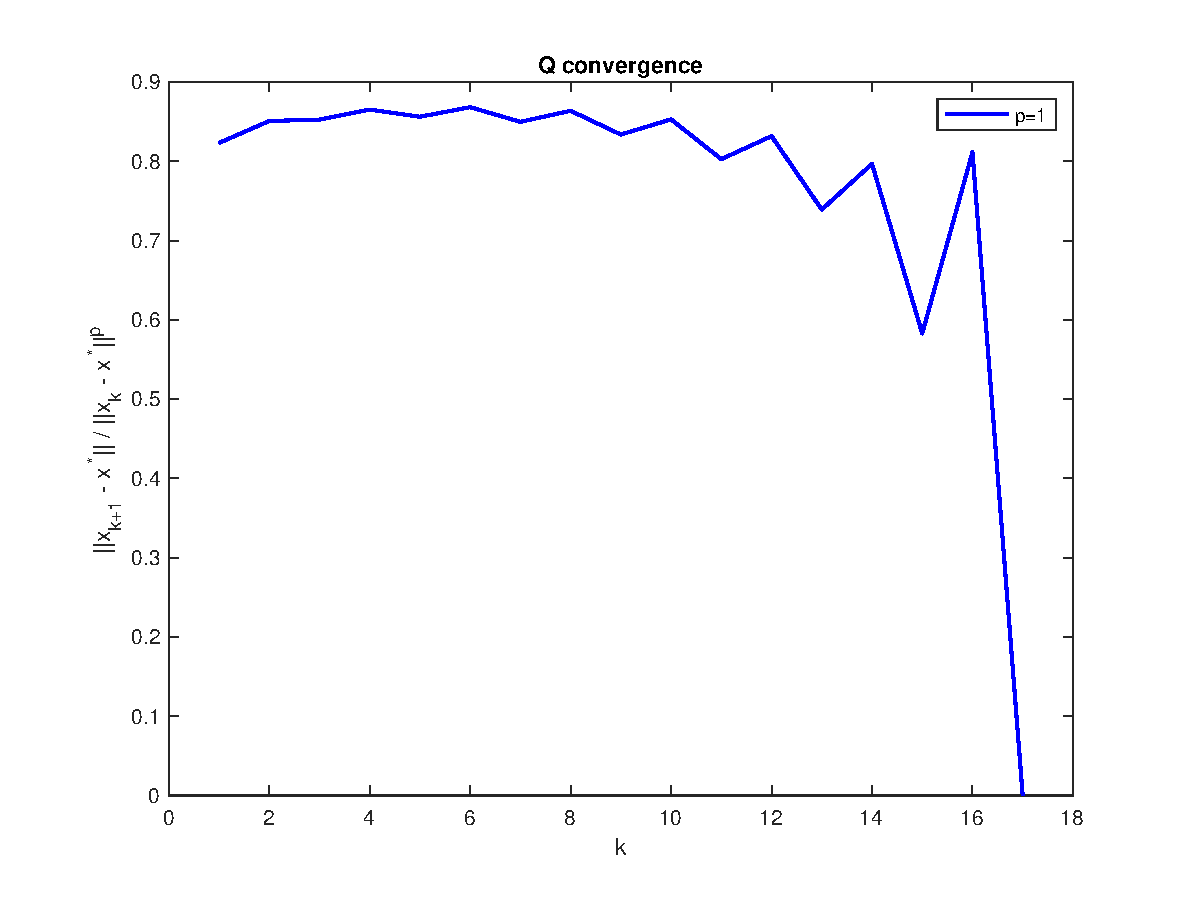
\includegraphics[width=0.85\textwidth]{Convergence.eps}
\end{center} \par


% ----------
% Part (c)
% ----------
\subsection*{Q3 – Part (c)}
Discussing the theoretical and empirical convergence rates is somewhat trivial in our circumstances. The specific reformulation of our primal (9) and dual (11) was designed to reduce the constraints, and therefore the number of checks, required to ensure our convergence rates matched that indicated by the theory. This is a result of the LSVM Algorithm falling into a specialist category of implementations by exploiting an alternative formulation of the optimisation problem itself \cite{cherkassky2007learning} – which is in contrast to other traditional algorithms such as SMO \cite{platt1998sequential} or SVM-\textit{light} \cite{joachims1999svmlight}. \par

We can, for the sake of completeness, perform the appropriate checks. Firstly, we must check that (28/29) holds, that is,
\begin{equation}
    0 \leq \tau \leq \frac{2}{\nu}.
\end{equation}

In the MATLAB implementation of the algorithm (see Appendix), we have specified $\tau = \frac{1.9}{\nu}$, thus for any value of $\nu$ parsed to the function the condition will be satisfied. \par

Secondly, we must check that the KKT necessary and sufficient conditions hold. We have seen from Q2 - Part (b), equations (22-25), that Mangasarian \cite{mangasarian1994nonlinear} developed the iterative steps of the algorithm using those conditions, thus they are satisfied by construction. \par

Finally, we know that both matrices $K$ and $M$ are positive by construction \cite{scholkopf2002learning:ch10}, hence, all assumptions of the Theorem 2.3 are satisfied, and the empirical convergence rate agrees with the theoretical.

% ----------
% Part (d)
% ----------
\subsection*{Q3 – Part (d)}
To discuss complexity, we return to the scenarios discussed in Q2 - Part (b). Under the best case, the low rank approximation and the Sherman-Woodbury-Morrison result in a dramatic reduction in complexity. For instance, the low-rank approximation means the inversion of $M$ is of order $O(n^{2}m)$ \cite{scholkopf2002learning:ch10}. Unfortunately, as our classification problem was unsuitable for this trick, our inversion of $M$ comes at the cost of order $O(m^3)$ \cite{scholkopf2002learning:ch10}. Once more indicating the LSVM method is only appropriate for small to intermediate sized problems. \par

The CPU time took an average of 21.23 seconds (using the same methodology described in part (b)), which is clearly good performance considering the complexity of the task. \par

The memory used, however, is disappointing but unsurprising. The storage of the matrix $M^{-1}$ required $195mb$, which is considerably higher than it would have been under the low-rank approximation. Whilst modern day computers are more than capable of efficiently handling these memory sizes, as well as complexity, the increase in memory used by the inverse matrix would become prohibitive for larger scale problems. 

% ----------
% Part (e)
% ----------
\subsection*{Q3 – Part (e)}
Of course, the ultimate purpose of SVMs is to classify datapoints. We now present the classification results of the LSVM method in the form of a confusion matrix and calculate the accuracy for the test set. Overall, we can see the LSVM Algorithm provides fast and accurate classification of dry beans.\par

\textbf{Confusion Matrix:} 
\begin{center}
    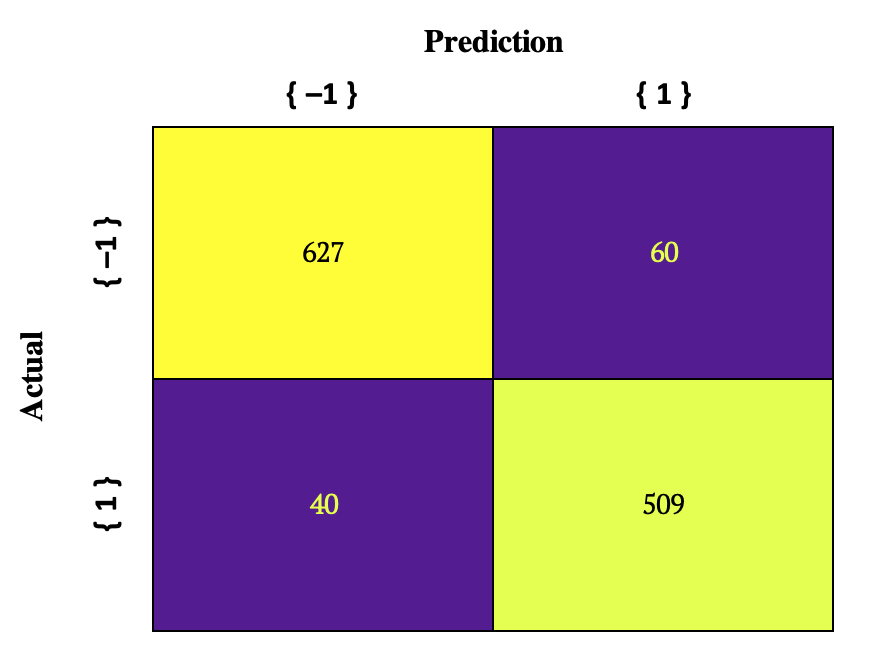
\includegraphics[width=0.65\textwidth]{Confusion Matrix.png}
\end{center} \par

\textbf{Accuracy: 91.91\%}




\newpage
\bibliographystyle{IEEEtran} % We choose the "plain" reference style
\bibliography{bibliography} % Entries are in the bibliography.bib file

\newpage
\begin{appendices}

\section*{Appendix}
\subsection*{Code: LSVM Implementation}
\small
\begin{verbatim}
    function [nIter, Opt, lambda1, w, tau, info] = nonLinLSVM(A,D,nu,maxIter,tol)

% Lagrangian Support Vector Machine Algorithm [NONLINEAR KERNEL]
%
% ------------------------------------------------
% Description:
% ------------------------------------------------
% An iterative algorithm that solves the dual problem with a non-linear 
% kernel, we can no longer use Sherman-Woodbury-Morrison, so must use
% in-built LU decomposition for inversion of the matrix. 
%
% ------------------------------------------------
% Inputs:
% ------------------------------------------------
%   A: The m x n input matrix of observations.
%      Where m = the number of observations in the dataset.
%            n = the number of features of the dataset.
%   D: The m x m matrix of the classifications on the diagonal {-1, 1}.
%   nu: Parameter required for bounding the eigenvalues.
%   maxIter: The maximum number of iterations accepted.
%   tol: The tolerance of the norms for each iteration.
%
% ------------------------------------------------
% Outputs:
% ------------------------------------------------
%   nIter: Number of iterations required.
%   Opt: Terminating norm.
%   lambda1: Vector satisfying the dual equation. Needs to be converted to
%   primal solution.
%   w: Orientation of our optimal hyperplane.
%   tau: Convergence parameter.
%   info: Structure for convergence plots.

% ================================================
%         ---------- ALGORITHM ----------
% ================================================

% Parameterization for simpler notation
m = size(A,1) ;
tau = 1.9/nu ;
one = ones(m,1) ;
I = speye(m) ;


% Kernel Computation
% K(H,H^T), where K is the kernel function
H = [A -one] ;

% KM: The kernel matrix, K_i,j = kernel(x_i,x_j). 
KM = (H*H').^2 ; % Quadratic Polynomial Kernel

% Compute required matrices
M = I/nu + D * KM * D;
P = inv(M);

info.Mlambda_steps = [] ;
info.M = M ; 

% Initialization
lambda1 = P*one ;
lambda0 = lambda1+1 ;
nIter = 0 ;

% Iterative loop
while nIter< maxIter && norm(lambda0-lambda1) > tol
    % Update the previous step
    lambda0 = lambda1 ;
    % Compute the next iteration
    lambda1 = P*(1+pos(M*lambda1-1-tau*lambda1)) ;
    % Capture path for convergence
    info.Mlambda_steps = [info.Mlambda_steps M*lambda1] ;
    % Increment 
    nIter = nIter+1 ;
end

% Outputs
Opt=norm(lambda1-lambda0);
w = A' * D * lambda1;
tau = -one' * D * lambda1;

% Function to account for the ((Mlambda_i - one) - tau lambda_i)_{+} 
% in the true iterative step (25)
%  --> pos(x) = { x , if x > 0
%  --> pos(x) = { 0 , if x < 0
function pos = pos(x)
pos = (abs(x)+x)/2;
\end{verbatim}

\newpage
\subsection*{Code: SVM Testing Script}
\small
\begin{verbatim}
%% Testing Script

% Define the parameters
% (As defined in Q2b and Q3a).
A = beans_trainX ;
nu = 1e-3 ;
maxIter = 1e3 ; 
tol = 1e-3 ;
D = diag(beans_trainY);


% Implementation of the non-linear LSVM Algorithm
[nIter, Opt, lambda1, w, tau, info] = nonLinLSVM(A,D,nu,maxIter,tol) ;

%% Computing the performance
% (Excluded for brevity)

\end{verbatim}

\end{appendices}


\end{document}
